\documentclass[tikz,border=2pt]{standalone}
\usepackage{amsmath}
\usetikzlibrary{arrows.meta}
\begin{document}
% Jobs offered at 1,4,5,8,9,12,13,16 (lambda = 1/2). Busy periods (red) for service time 1.5 (utilization 0.75),
% service time 2.5 without blocking (busy from t = 4 on, utilization 1) and 2.5 with blocking of jobs that find
% the server busy (jobs at 5, 9, 13 blocked; utilization 0.625).
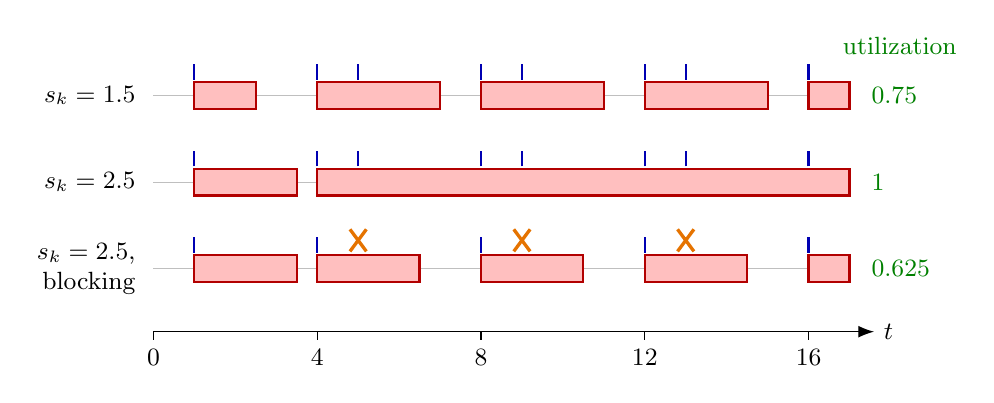
\begin{tikzpicture}[font=\small, >={Latex[length=2mm]}, x=0.52cm, y=1cm]
  \def\rowA{0} \def\rowB{-1.1} \def\rowC{-2.2}
  % baselines
  \foreach \r in {\rowA,\rowB,\rowC} {\draw[gray!50] (0,\r) -- (17,\r);}
  % busy periods
  \foreach \a/\b in {1/2.5, 4/7, 8/11, 12/15, 16/17} {
    \fill[red!25] (\a,\rowA-0.17) rectangle (\b,\rowA+0.17); \draw[red!70!black, thick] (\a,\rowA-0.17) rectangle (\b,\rowA+0.17);}
  \foreach \a/\b in {1/3.5, 4/17} {
    \fill[red!25] (\a,\rowB-0.17) rectangle (\b,\rowB+0.17); \draw[red!70!black, thick] (\a,\rowB-0.17) rectangle (\b,\rowB+0.17);}
  \foreach \a/\b in {1/3.5, 4/6.5, 8/10.5, 12/14.5, 16/17} {
    \fill[red!25] (\a,\rowC-0.17) rectangle (\b,\rowC+0.17); \draw[red!70!black, thick] (\a,\rowC-0.17) rectangle (\b,\rowC+0.17);}
  % arrivals
  \foreach \r in {\rowA,\rowB} {\foreach \t in {1,4,5,8,9,12,13,16} {\draw[blue!70!black, thick] (\t,\r+0.2) -- (\t,\r+0.4);}}
  \foreach \t in {1,4,8,12,16} {\draw[blue!70!black, thick] (\t,\rowC+0.2) -- (\t,\rowC+0.4);}
  \foreach \t in {5,9,13} {\draw[orange!90!black, very thick] (\t-0.2,\rowC+0.22) -- (\t+0.2,\rowC+0.5) (\t-0.2,\rowC+0.5) -- (\t+0.2,\rowC+0.22);}
  % row labels
  \node[anchor=east] at (-0.2,\rowA) {$s_k=1.5$};
  \node[anchor=east] at (-0.2,\rowB) {$s_k=2.5$};
  \node[anchor=east, align=right] at (-0.2,\rowC) {$s_k=2.5$,\\ blocking};
  \node[green!50!black, anchor=west] at (17.3,\rowA) {$0.75$};
  \node[green!50!black, anchor=west] at (17.3,\rowB) {$1$};
  \node[green!50!black, anchor=west] at (17.3,\rowC) {$0.625$};
  \node[green!50!black, anchor=south west] at (16.6,\rowA+0.4) {utilization};
  % time axis
  \draw[->] (0,-3.0) -- (17.6,-3.0) node[right] {$t$};
  \foreach \t in {0,4,8,12,16} {\draw (\t,-3.0) -- (\t,-3.1) node[below] {$\t$};}
\end{tikzpicture}
\end{document}
